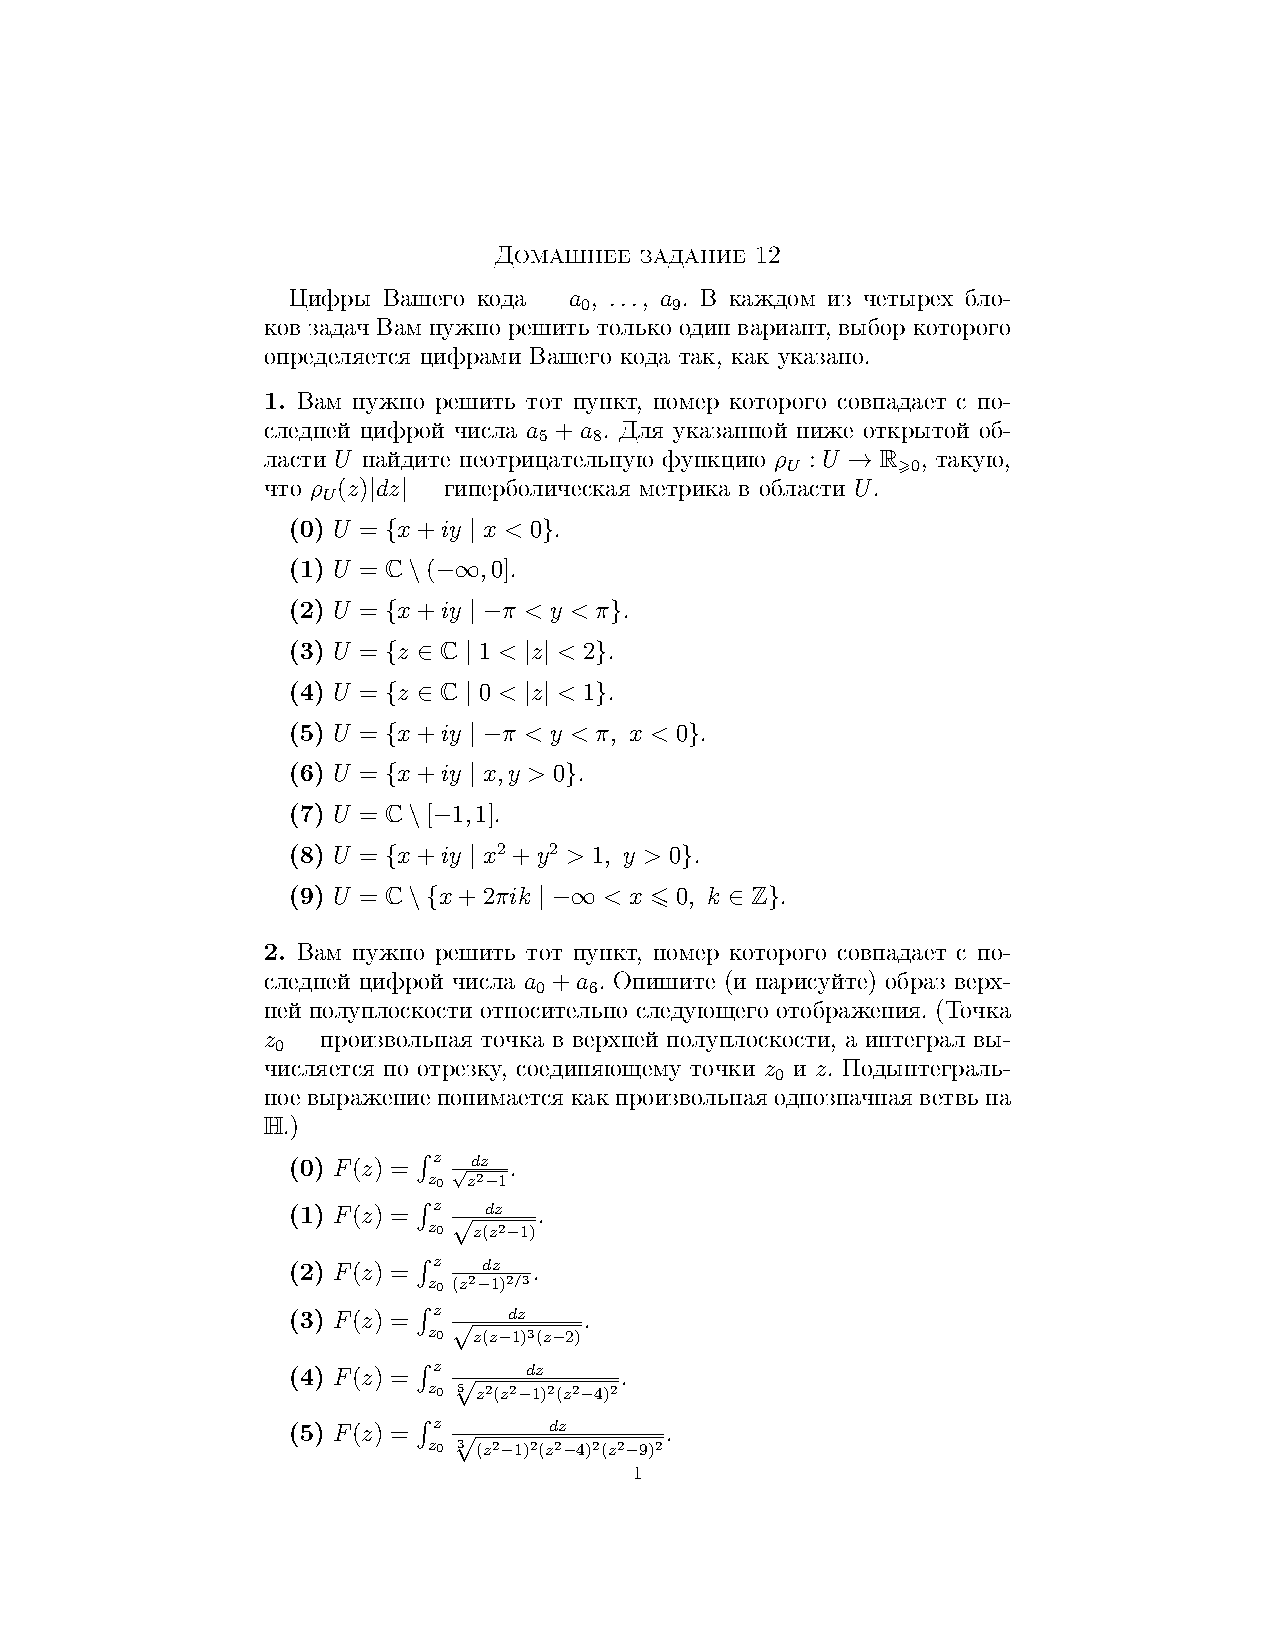
\includepdf[scale=1,pages=1-3]{Tasks/hw12}
\newpage
\section*{Решения}
\subsection*{Задача 1}
	Необходимо решить задачу $a_5 + a_8 = 6 + 8 = 4 \mod 10$\\
\vskip 0.4in

\subsection*{Задача 2}
	Необходимо решить задачу $a_0 + a_6 = 1 + 9 = 0 \mod 10$\\
	Представим $F(z) = \int_{z_{0}}^{z} \frac{dz}{\sqrt{z^2 - 1}}$ как $F(z) = \int_{z_{0}}^{z} \frac{dz}{\sqrt{(z - 1)(z + 1)}}$. Заметим, что $f(z_0) = 0$
\vskip 0.4in

\subsection*{Задача 3}
	Необходимо решить задачу $a_2 + a_5 = 8 + 6 = 4 \mod 10$\\
	Заметим, что $\cos(e^z - \sin(z))$ аналитична и имеет существенную особенность на бесконечности, а следовательно, по теореме Пикара, она принимает все значения, кроме одного, в данной окрестности бесконечно много раз, а следовательно
	 так как у $\cos(e^z - \sin(z)) - 2$ есть 1 корень, то корней бесконечно много
\vskip 0.4in

\subsection*{Задача 4}
	Необходимо решить задачу $a_8 + a_9 = 8 + 6 = 4 \mod 10$\\
	

